\section{Contribuindo com plataformas abertas} % (fold)
\label{sec:contribuindo_com_plataformas_abertas}

Um dos intuitos deste trabalho baseia-se em contribuir com uma aplicação \textit{open-souce} disponível na plataforma \href{GitHub.com}{GitHub}. A seguinte sessão se destina em apresentar a forma como tais contribuições podem ser realizadas. Devido ao repositório do APT esta armazenado no GitHub, a sessão pode se tornar tendenciosa, porém o conceito de \textit{pull-request} ou  \textit{merge-request} requeste é amplamente utilizado em outras plataformas de contribuição, como \href{https://bitbucket.org/}{Bitbucket}, \href{https://gitlab.com/}{GitLab} ou ate mesmo \href{http://sourceforge.net/}{SourceGorge}.


\subsection*{Mantendo uma copia} % (fold)
\label{sub:mantendo_uma_copia_sua}


Normalmente não temos autorização pra alterar as informações de outra pessoa sem seu consentimento. Da mesma forma  é com os repositórios {\code git}. Assim, um dos primeiros passos para começar a contribuir com uma ferramenta \textit{open-source} é fazer uma copia dela em seu repositório. Essa cópia pode ser feita de duas formas basicamente, no intuito de manter os autores das modificações anteriores:

\begin{description}
	\item [\textit{Fork}]: O termo é amplamente utilizado quando queremos fazer uma copia de um repositório para a nossa conta em uma mesma plataforma. Normalmente este passo é realizado via interface gráfica, ainda no navegador. Na \cref{fig:github_fork} é possível observar o botão no canto superior direito indicado para realizar um \textit{fork} do atual repositório.

	\begin{figure}[h]
	  \centering
		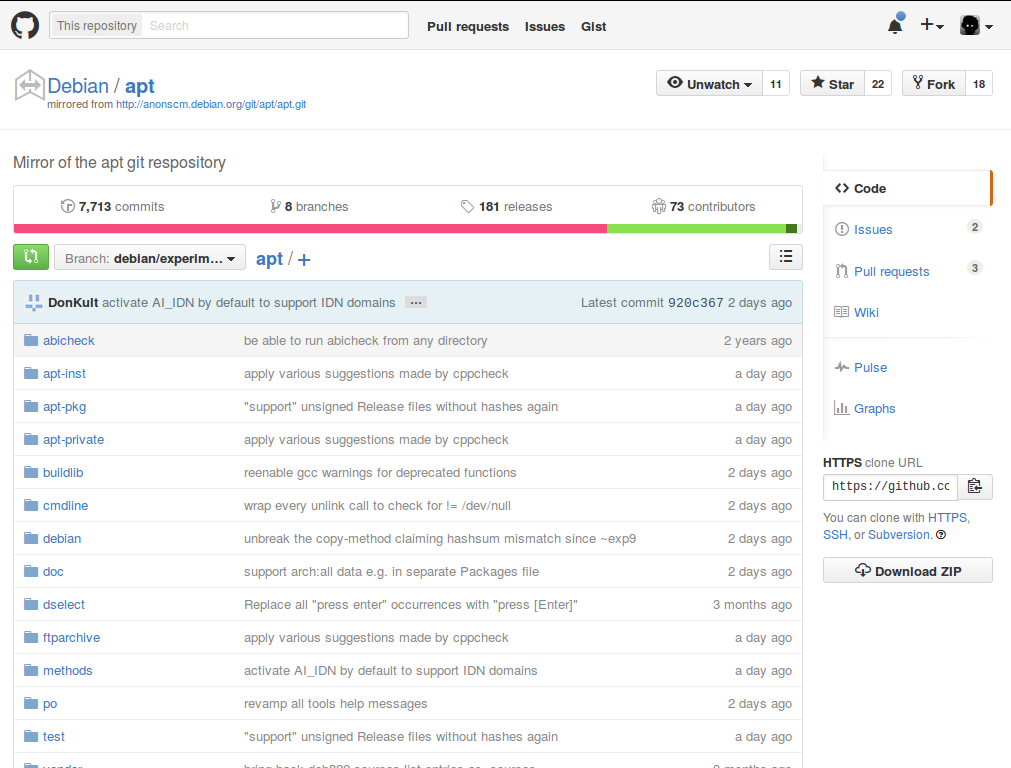
\includegraphics[width=0.85\textwidth]{figuras/fork}
	  \caption{Visão de um repositório do \textit{GitHub}}
	  \label{fig:github_fork}
	\end{figure}

	\item [\textit{Adicionando \textit{remote}}]: Quando desejamos realizar uma copia do repositório em uma plataforma distinta da original, a forma mais simples de proceder é clonando o repositório e incluindo nele um novo \textit{remote} para a nova plataforma. Assim conseguimos trabalhar com a mesma arvore de \textit{commits} do repositório original, mantendo os créditos e alterações originais.
\end{description}
% subsection mantendo_uma_copia_sua (end)

\subsection*{Evoluindo o código} % (fold)
\label{sub:evoluindo_o_c_digo}

Nesto ponto de contribuição, o contribuinte desenvolve o código semelhante ao processo de produção de código pessoal. O código já esta em um repositório pessoal e o usuário já possui todos os direitos administrativos do repositório. Obviamente que caso a contribuição esteja sendo feita à uma aplicação grande e com muitos contribuidores, é importante se manter sincronizado com o código original, para evitar que o retorno da contribuição não seja tão trabalhoso para o revisor, além de evitar situações de conflitos.
% subsection evoluindo_o_c_digo (end)

\subsection*{Retornando sua contribuição} % (fold)
\label{sub:retornando_sua_contribui_o}

Quando se decidido que a contribuição já esta a um ponto aceitável para encaminha-la de volta para o código original, é o momento de se realizar o \textit{pull-request}\footnote{Ou \textit{merge-request} dependendo do ambiente de desenvolvimento em que esteja-se contribuindo.}. Uma contribuição é interessante quando possui as seguintes características:


\begin{itemize}
	\item Evolução de código mantendo os padrões de guia de estilo definido pelo desenvolvedor original/linguagem.
	\item Testes para a evolução de código proposto.
	\item Documentação da \textit{feature} implementada ou atualização da documentação como reflexão das modificações sugeridas.
\end{itemize}
% subsection retornando_sua_contribui_o (end)

Realizada a contribuição, é dever do mantenedor do repositório original revisar o código e decidir se deve ou não aceita-lo.

% section contribuindo_com_plataformas_abertas (end)


\section{Coleta de Dados} % (fold)
\label{cha:coleta_de_dados}

\subsection*{Tempo} % (fold)
\label{sec:tempo}

A coleta de tempo de performance de um software é árdua. A estimativa de tempo depende das otimizações que o compilador pode vir a fazer para a arquitetura, memoria disponível, aplicativos rodando em concorrência, temperatura do hardware, etc. No intuito de simplificar o processo de estimativa de tempo, foi utilizado a mediana de uma serie de chamadas da aplicação. Segundo \citeonline{dolan2002benchmarking}, esta solução pode vir ser a melhor para um ponto geral de $25\%$ das possíveis alternativas de coletas de dados. Assim sendo, o \autoref{scriptods} foi uma solução desenvolvida que permitisse deixar a maquina com tempo dedicado para a aquisição de dados.

Para o funcionamento do \textit{script}, as variáveis {\code MAX} e {\code \_MAX\_THREADS} devem ser definidas com a quantidade de dados que se deseja coletar e a quantidade máxima de \textit{threads} que devem ser levantadas para a chamada do processo respectivamente. Usar uma quantidade superior a quantidade de \textit{cores}  da maquina pode produzir valores com baixa confiabilidade, visto a concorrência gerada pelas \textit{threads}. Como parâmetros, foram escolhidos $150$ dados com $7$ \textit{threads}, possibilitando haver ao menos $1$ \textit{core} livre. Para maior dinamismo da coleta dos dados, o \textit{script} é responsável por realizar a troca das \textit{branchs} onde estão localizadas as possíveis soluções e a compilação e concentração dos dados em uma planilha do \textit{LibreOffice Calc}. Assim, os algoritmos nunca são executados em concorrência, porém os dados serão coletado sob a demanda da $CPU$ em que o \textit{script} é executado.

No intuito de coletar o tempo pontual do algoritmo, o \autoref{libtime} foi desenvolvido a fim de ser usado como cronometro. O algoritmo desenvolvido com o auxilio da biblioteca {\code Chrono}\footnote{A biblioteca é disponibilizada no {\code C++11} sob o \textit{namespace} {\code std::crono::}.} permite a captura do intervalo de tempo com ate $9$ casas decimais de segundos (nanosegundos), todavia foi utilizado a precisão de microssegundos apenas, visto que o intervalo de nanosegundos não iria gerar alto impacto na diferença dos valores. Os métodos {\code begin} e {\code end} da classe são utilizados para pontuar os intervalos onde o tempo deve ser contado. O resultado da contagem pode ser obtido com o retorno do método {\code end} ou com a chamada do {\code currenttime}, dedicado apenas para o retorno deste valor.

\subsection*{Memória}

Para a coleta de memória, foi utilizado o {\code Valgrind} com o auxilio da ferramenta {\code Massif}. Devido a haver uma criação de \textit{hash} de forma  algébrica e o método de \textit{KMP} faz uso de um autômato finito determinístico, a previa repetição das buscas com apenas $10$ ciclos confirmavam a suspeita de não haver a variação do gasto de memória para a repetição da ação.

Para a execução da aplicação com o suporte do {\code Valgrind} para analise do uso de memória, foi utilizado o seguinte comando:

\begin{lstlisting}[language=Bash,label=valgrind_call, numbers=none]
   $ valgrind --tool=massif  ./apt search pacote [--regex]
\end{lstlisting}
% section tempo (end)
% chapter coleta_de_dados (end)


\section{Primeira contribuição} % (fold)
\label{sec:primeira_contribui_o}

A primeira contribuição tinha como objetivos a ambientalização com o ambiente e o time oficial de desenvolvimento. Como tarefa, foi definido a implementação minima de uma estrutura que permita um contexto de ordenação que possa ser definido pelo usuário. O intuito era oferecer as seguintes opções de ordenação na primeira contribuição:

\begin{description}
	\item [\textit{Alphabetic}] Ordenação padrão em ordem alfabética. Os pacotes são ordenados de acordo com seu nome.
	\item [\textit{Reverse Alphabetic}] Semelhante a ordenação alfabética, porém em ordem decrescente, ou seja, palavras que começam com {\code Z} são apresentadas antes das iniciadas com {\code A}.
	\item [\textit{Status}] Ordena os pacotes de acordo com as seguintes características:
	\begin{enumerate}
		\item Desinstalado,
		\item Instalado e com possível atualização,
		\item Instalado via pacote local,
		\item Instalado e descartável (auto removível),
		\item Instalado automaticamente,
		\item Instalado,
		\item Atualizável,
		\item Com configuração residual
	\end{enumerate}
	\item [\textit{Version}] Ordena a saída de acordo com a versão da aplicação.
\end{description}

\subsection*{Alteração da estrutura de dados} % (fold)
\label{sub:altera_o_da_estrutuda_de_dados}

Originalmente, os dados eram armazenados em um {\code map}, visto que essa estrutura não permite a duplicação de chaves e possui uma ordenação alfabética automática. Todavia, alterar o algoritmo de ordenação de um {\code map} ocorrem em seu tempo de declaração, o que  inviabiliza a possibilidade de alterar a ordenação através de uma \textit{flag} como parâmetro de execução. Visto essa condição, a estrutura foi alterada para a estrutura de dados {\code vector}, por ser mais flexiva quanto a sua forma de ordenação.

Naturalmente, a inserção de candidatos na saída do APT ocorre  em dois níveis. O primeiro ordena de acordo com os repositórios inseridos no {\code source.list} da distribuição. Candidatos de um mesmo repositório serão naturalmente ordenados alfabeticamente. Isso implica que apenas adicionar candidatos no vetor implicaria em uma ordenação com baixa precisão, visto que a sequência de repositórios variaria de usuário para usuário. Assim, a simples troca de estrutura de dados de {\code map} para {\code vector} implica na necessidade de implementar o método de ordenação alfabética, antes nativamente implementado pela estrutura {\code map}.

Tendo um método para ordenação alfabética simplifica o processo de ordenação alfabético reverso, visto que basta enviar as referências do vetor com suas reversas, ao invez da normais. Assim, bastando ser necessário a escrita de três métodos no total para a primeira contribuição. No trecho de código a seguir é apresentado como a seleção de ordenação é tomada.


\begin{lstlisting}[language=C++,label=choose_pr1,caption={Tomada de decisão de ordenação}]
   switch(PackageInfo::getOrderByOption())
   {
      case PackageInfo::REVERSEALPHABETIC:
		 std::sort(outputVector.rbegin(), outputVector.rend(), OrderByAlphabetic);
		 break;
      case PackageInfo::STATUS:
			 std::sort(outputVector.begin(), outputVector.end(), OrderByStatus);
			 break;
      case PackageInfo::VERSION:
		 std::sort(outputVector.begin(), outputVector.end(), OrderByVersion);
		 break;
      default:
		 std::sort(outputVector.begin(), outputVector.end(),   OrderByAlphabetic);
		 break;
   }
\end{lstlisting}

A versão apresentada neste trabalho é o resultado de alguns \textit{feedback} sugeridos pelos mantenedores do projeto, em especial \href{https://github.com/DonKult}{David Kalnischkies}, o qual fez questão de pontuar detalhes na contribuição que poderiam ser melhorados ou questionados\footnote{David Kalnischkies não via muito sentido em uma ordenação por \textit{status}, porém não vetou a contribuição, visto que este pedido havia sido feito pelo membro \href{https://github.com/mvo5}{Michael Vogt} nos comentários da versão original do código.} no processo de aceitação da contribuição.

% subsection altera_o_da_estrutuda_de_dados (end)

\subsection*{Testando alterações} % (fold)

Realizar uma contribuição sem seus testes implica em oferecer um trabalho sem garantias de funcionalidade. Desta forma, as contribuições realizadas neste trabalho também estão sempre acompanhadas de seus respectivos testes. O APT utiliza uma ferramenta de testes muito comum em $C++$, a \textit{Google Test}\footnote{Mais informações sobre a ferramenta podem ser obtidas em seu repositório oficial: \url{https://github.com/google/googletest}.}. Uma \textit{suite} de testes é caracterizada pelo \textit{Google Test} como um arquivo contendo $n$ testes. Para manter o contexto, as condições da \textit{suite} de testes deve ser definida no inicio.

\begin{lstlisting}[language=Bash,label=googletest_decl,caption={Declarações de instâncias para o teste}]
setupenvironment
configarchitecture "i386"

DESCR='Some description that has a unusual word xxyyzz and aabbcc and a UPPERCASE'
DESCR2='Some other description with the unusual aabbcc only'
DESCR3='Some package description'
DESCR4='an autogenerated dummy baz=0.1/installed'
insertpackage 'unstable' 'foo' 'all' '1.0' '' '' "$DESCR
 Long description of stuff and such, with lines
 .
 and paragraphs and everything."
insertpackage 'testing' 'bar' 'i386' '2.0' '' '' "$DESCR2"
insertpackage 'stable' 'package' 'all' '1.5' '' '' "$DESCR3"
insertinstalledpackage 'baz' 'all' '0.1'

setupaptarchive
\end{lstlisting}

Como apresentado no código \ref{googletest_decl}, algumas macros foram criadas pela equipe do APT para simplificar o processo de declaração de instâncias. Com estas instâncias declaradas, o contexto do teste é estabelecido e esta pronto para a \textit{suite} de testes rodarem. Os testes são basicamente cenários do estado do sistema, como pode ser observado no código \ref{gtest_foo}.

\begin{lstlisting}[language=Bash,label=gtest_foo,caption={Teste por busca pelo pacote \textit{foo}}]
# search name
testsuccessequal "foo/unstable 1.0 all
  $DESCR
" apt search -qq foo
\end{lstlisting}

Como estamos fazendo ordenação de pacotes, é importante que se possa realizar uma busca por uma grande quantidade de pacotes. Uma das possibilidades que o APT possui hoje é a de se realizar buscas utilizando de expressões regulares. Unindo esta duas características, podemos montar uma lista maior de pacotes e realizar uma busca por um termo genérico, a fim de obter como resultado toda a lista de pacotes. O exemplo o código \ref{buscacomregex} demostra este resultado, onde a busca é feita utilizando a \textit{regex} {\code \textbackslash w}, a fim de selecionar todos os pacotes que possuam ao menos um caractere no nome.

\begin{lstlisting}[language=Bash,label=buscacomregex,caption={Busca com uso de expressão regular}]
# output is sorted by status
testsuccessequal "bar/testing 2.0 i386
  $DESCR2

foo/unstable 1.0 all
  $DESCR

package/stable 1.5 all
  $DESCR3

baz/now 0.1 all [installed,local]
  $DESCR4
" apt search --order-by status -qq "\\w"
\end{lstlisting}

% section primeira_contribui_o (end)


\section{Segunda contribuição} % (fold)
\label{sec:segunda_contribui_o}

O suporte a expressões regulares amplia como a busca por pacotes pode ser efetuada, possibilitando uma maior gama de ferramentas para desenvolvedores experientes. Todavia, deixar essa opção como padrão acarretam em alguns pontos negativos que são desempenhados todas as vezes que a aplicação é executada:

\begin{description}
	\item [Alto consumo de memoria:] Buscas com expressões regulares consomem cerca de $\Theta(2^n)$ para uma expressão de tamanho $n$, ou $\Theta(n^2)$ para melhores casos, com hardware dedicado\cite{sidhu2001fast}.
	\item [Baixo desempenho:] Buscas com expressões regulares tem custo de desempenho $\Theta(n)$, sendo $n$ o tamanho da palavra a ser analisada.
\end{description}

Mesmo a busca com expressões regulares oferecendo um grande poder de busca, questiona-se se o custo que ela requer é interessante. Lembrando que este trabalho visa ampliar a comodidade daqueles novos usuário ao mundo Linux, as funções de expressões regulares normalmente não são de conhecimento do usuário leigo. Considerando que este usuário leigo não irá fazer comumente das funções {\code less}, {\code more} ou {\code grep} para auxiliar com buscas, será de menor representatividade então o uso de expressões regulares.

% Ora, se há a possibilidade de ganhar desempenho e gasto de memoria mesmo ainda com busca exatas, há de se propor algoritmos para nos auxiliar com essas buscas.


Visando uma alternativa para a busca de pacotes que ofereça menor tempo de processamento e maior economia de memoria, foram estudados dois algoritmos de \textit{string matching} exato abordados inicialmente neste trabalho na \autoref{sec:algoritimos_de_textit}, são os modelos de \nameref{ssub:rabin_karp} e \nameref{ssub:knuth_morris_pratt_}. Para ambos os modelos foram criadas \textit{branchs} para seu desenvolvimento e testes de desempenho, fazendo de uso da rotina apresentada no \autoref{libtime} para mensurar o tempo gasto para formular a resposta da pesquisa. 

Diante dos resultados de tempo obtidos com o algoritmo de \textit{Rabin-Karp}, a segunda contribuição foi planejada e executada. A \autoref{sec:segundo_pr} apresenta na integra o \textit{diff} da contribuição submetida para o repositório oficial.


A fim de manter a cobertura das funcionalidades, testes foram feitos para garantir que as buscas continuavam a ser realizadas com ou sem o uso da \textit{flag} que habilitava o uso de expressões regulares, como pode ser observado no \autoref{regextestscli}, onde um trecho dos testes da segunda submissão é apresentado.

\begin{lstlisting}[language=Bash,label=regextestscli,caption={Teste com e sem o uso de expressões regulares}]
# output is sorted by status
testequal "bar/testing 2.0 i386
  $DESCR2

foo/unstable 1.0 all
  $DESCR

package/stable 1.5 all
  $DESCR3

baz/now 0.1 all [installed,local]
  $DESCR4
" apt search --order-by status -qq "\\w" --regex

# output is sorted by Alphabetic (non case sense)
testequal "bar/testing 2.0 i386
  $DESCR2

baz/now 0.1 all [installed,local]
  $DESCR4
" apt search --order-by Alphabetic -qq ba
\end{lstlisting}

Garantido haver testes e documentação que validem as implementações, foi realizado a submissão de \textit{merge request} ao repositório oficial do APT, a qual pode ser observada na \autoref{fig:pr2_travisok} e acompanhada em \url{https://github.com/Debian/apt/pull/8}.

\begin{figure}[h]
  \centering
	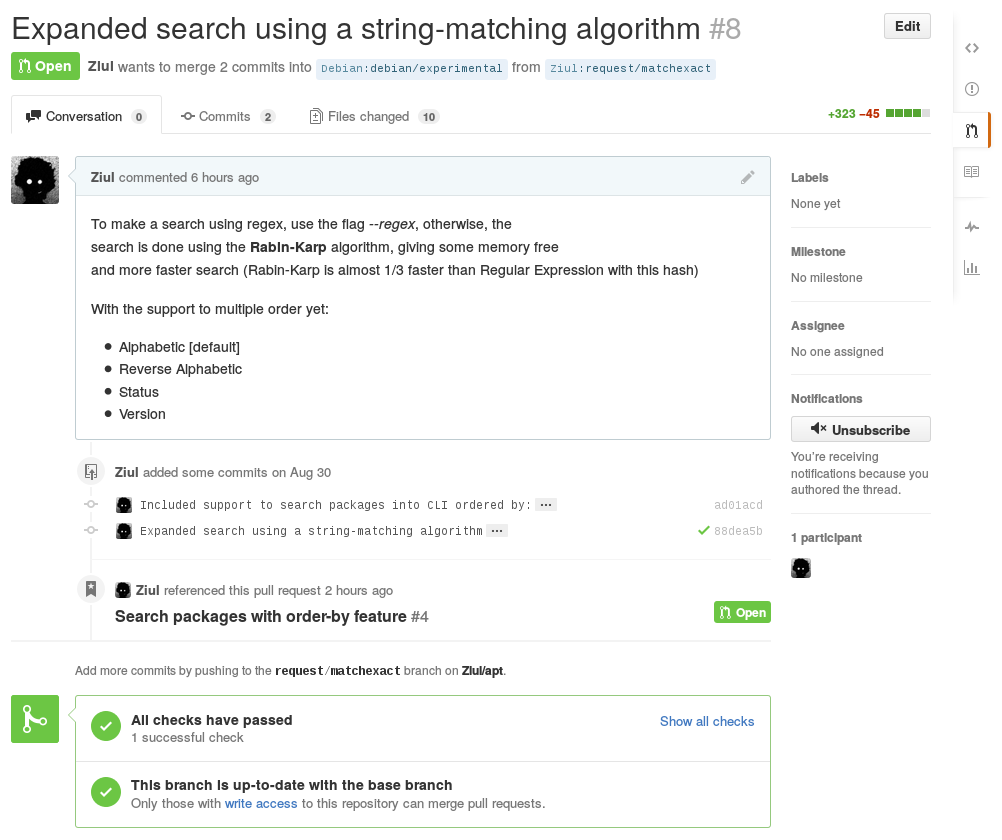
\includegraphics[width=0.95\textwidth]{figuras/pr2}
  \caption{Submissão do segundo \textit{merge request}}
  \label{fig:pr2_travisok}
\end{figure}

% section segunda_contribui_o (end)

\section{Terceira contribuição} % (fold)
\label{sec:terceira_contribui_o}

Por fim chegamos ao ponto desejado para este trabalho, oferecer uma ferramenta de busca de pacotes o mais transparente possível quanto ao método de busca. Para tal precisamos ainda realizar duas tarefas:

\begin{description}
	\item [Escolha inteligente entre expressões regulares ou busca padrão:] Mesmo oferecendo uma \textit{flag} para selecionar a busca com suporte a expressões regulares, é importante deixar que o programa seja capaz de identificar quando uma \textit{flag} é passada para que a busca seja realizada corretamente.
	\item [Inserir método de buscas inexatas:] Quando uma busca não obtiver nenhum resultado, a aplicação deve executar a busca novamente com o método de buscas inexatas e apontar os pacotes que poderiam se encaixar com a busca realizada.
\end{description}

Para realizar a primeira tarefa devemos primeiro implementar uma função que verifique se entre os parâmetros passados na busca há um caractere especial utilizado para expressões regulares. Estes caracteres deveriam de ser {\code |\textbackslash\{\}[]()*+-\$?.\^{}}, porém os caracteres {\code .} e {\code -} costumam aparecer nos nomes dos pacotes e assim devem ser ignoradas como sinais que indicam uso de expressões regulares.
O \autoref{regexidentify} apresenta uma solução para a identificação de caracteres que indicam o uso de expressões regulares nas buscas.

\begin{lstlisting}[language=C++,label=regexidentify,caption={Identificação de Expressões Regulares}]
	
\end{lstlisting}



% section terceira_contribui_o (end)
